\documentclass[a4paper,12pt]{article}
\usepackage{../common/style_exercise}
\input{../common/definitions}
% --- packages for the Section 4 supplement (latent-variable models) ---
\usepackage{amsmath,amssymb,booktabs,graphicx}
\usepackage{tikz}
\usetikzlibrary{positioning,arrows.meta,fit,calc}
\graphicspath{{img/exercise03/}}
\usepackage[nameinlink]{cleveref}

\begin{document}
\names % header snippet with names of all facilitators of the exercises, see style_exercise.sty for details and adapt accordingly
\header{3}{\textbf{[TBD]} January 2027} % put here # of exercise   % TODO(dates): set the exact hand-in date for WS 2026/27

In this exercise, we will go through several aspects of calorimetry in high energy physics. 
We will start with the basic concepts related to the interaction of particles with matter and how they are exploited to perform energy measurements.
Then, we will use simulated events in a calorimeter with the geometry of the \href{https://www.phenix.bnl.gov/}{PHENIX} electromagnetic calorimeter to visualize some examples of what we can expect to observe in a real experiment.
Each particle typically deposits energy in several channels of a calorimeter, which introduces the problem of how to associate each energy deposit to the correct particle, and how to correctly count how many particles deposited energy in the calorimeter.
Clustering algorithms are fundamental tools to fulfill this task: we will introduce the k-means algorithm, a relatively simple and intuitive algorithm to perform clustering.
We will guide you through the implementation of the k-means algorithm, and you will compare your own creation with the implementation available in scikit-learn!
We will then introduce a more realistic approach, based on the seeding of clusters.
Finally, Section~4 connects k-means to the Expectation-Maximization algorithm and to Variational Autoencoders (see the pages after this one).

% TODO(dates): replace the two [TBD] placeholders below with the WS 2026/27 dates
As you will quickly notice, the notebook has a lot of content: we know this. The hand-in and review will be in January 2027 (\textbf{exact date: [TBD]}), and we will offer one session where you can collect your questions and doubts in November 2026 (\textbf{date and time: [TBD]}).

To start with the exercise, please login to the \href{https://jupytermachine.etp.kit.edu}{jupytermachine}, 
start the standard \texttt{Datenanalyse} container and update your \texttt{tp1\_forstudents} repository, 
e.g. by navigating to the directory in the file browser on the left and then selecting \texttt{Git -> Pull from Remote} from the menu bar. 
A new subfolder \texttt{Exercise03} should appear with a Jupyter notebook \texttt{Exercise03.ipynb}. 
Open the notebook and work through the different tasks that are given inside.

% =====================================================================
% Section 4 supplement: latent-variable models (K-means -> EM -> VAE)
% =====================================================================
\newpage
\sloppy % long code names and links in this supplement
\section*{Section 4: Latent-variable models --- from $k$-means to EM to VAE}
\addcontentsline{toc}{section}{Section 4: Latent-variable models}

The last section of the notebook revisits the clustering problem from the point of view of \emph{latent-variable models}, following the lecture
``Variational Autoencoder'' (K.~He, MIT 6.S978 \emph{Deep Generative Models}, 2024).
You will see that the $k$-means algorithm of Section~3, the Expectation-Maximization (EM) algorithm and the Variational Autoencoder (VAE) are three ways of
maximising one and the same objective, and you will use them for three calorimetry tasks:
sharing the energy of overlapping showers, choosing the number of clusters, and learning what a ``normal'' electromagnetic shower looks like.

\subsection*{The generative picture}

A latent (hidden) variable $z$ is drawn from a prior $p(z)$ and a generator produces the observation, $x\sim p_\theta(x\,|\,z)$.
In a calorimeter this is the physics itself: for a single \emph{hit}, $z$ says which particle produced it and $p_\theta(x|z)$ is the lateral shower profile around the impact point;
for a whole \emph{shower}, $z$ contains the impact point, energy and shape, and $p_\theta(x|z)$ is the electromagnetic cascade plus the detector response.
For any distribution $q(z)$ the log-likelihood can be decomposed as
\begin{equation}
\log p_\theta(x) \;=\; \underbrace{\mathbb{E}_{q(z)}\big[\log p_\theta(x\,|\,z)\big] - D_\mathrm{KL}\big(q(z)\,\|\,p(z)\big)}_{\text{ELBO}(q,\theta)}
\;+\; \underbrace{D_\mathrm{KL}\big(q(z)\,\|\,p_\theta(z\,|\,x)\big)}_{\geq 0},
\label{eq:elbo}
\end{equation}
so the \emph{evidence lower bound} (ELBO) is a lower bound on $\log p_\theta(x)$, which becomes tight when $q$ equals the posterior $p_\theta(z|x)$.
The three methods differ only in how they represent $q$ and how they maximise the ELBO (\cref{tab:methods,fig:schematic}).

\begin{table}[h]
\centering
\small
\setlength{\tabcolsep}{5pt}
\begin{tabular}{@{}llll@{}}
\toprule
 & representation of $q(z)$ & maximisation of the ELBO & latent $z$ \\
\midrule
$k$-means & one-hot (hard) assignment & alternate: assign / update & discrete \\
EM (Gaussian mixture) & exact posterior (soft) & alternate: E-step / M-step & discrete \\
VAE & encoder network $q_\phi(z\,|\,x)$ & stochastic gradient descent & continuous \\
\bottomrule
\end{tabular}
\caption{Three ways to maximise the ELBO of \cref{eq:elbo}.}
\label{tab:methods}
\end{table}

\begin{figure}[h]
\centering
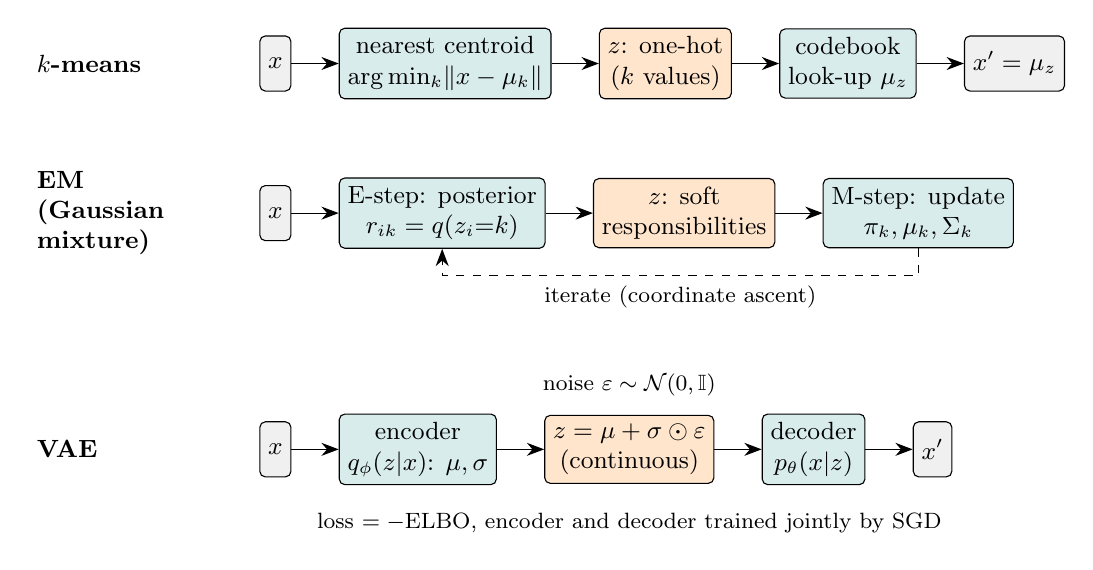
\begin{tikzpicture}[
  font=\small, >={Stealth[length=2.2mm]},
  box/.style={draw, rounded corners=2pt, minimum height=7mm, align=center, inner sep=3pt},
  dat/.style={box, fill=gray!12},
  lat/.style={box, fill=orange!20},
  net/.style={box, fill=teal!15},
  lab/.style={font=\small\bfseries, anchor=west, text width=2.4cm}]
  % k-means as an autoencoder
  \node[lab] (L1) at (-1.2, 0) {$k$-means};
  \node[dat, right=0.3cm of L1] (x1) {$x$};
  \node[net, right=0.6cm of x1] (e1) {nearest centroid\\$\arg\min_k \lVert x-\mu_k\rVert$};
  \node[lat, right=0.6cm of e1] (z1) {$z$: one-hot\\($k$ values)};
  \node[net, right=0.6cm of z1] (d1) {codebook\\look-up $\mu_z$};
  \node[dat, right=0.6cm of d1] (y1) {$x'=\mu_z$};
  \draw[->] (x1) -- (e1); \draw[->] (e1) -- (z1); \draw[->] (z1) -- (d1); \draw[->] (d1) -- (y1);
  % EM
  \node[lab] (L2) at (-1.2, -1.9) {EM\\(Gaussian mixture)};
  \node[dat, right=0.3cm of L2] (x2) {$x$};
  \node[net, right=0.6cm of x2] (e2) {E-step: posterior\\$r_{ik}=q(z_i{=}k)$};
  \node[lat, right=0.6cm of e2] (z2) {$z$: soft\\responsibilities};
  \node[net, right=0.6cm of z2] (d2) {M-step: update\\$\pi_k,\mu_k,\Sigma_k$};
  \draw[->] (x2) -- (e2); \draw[->] (e2) -- (z2); \draw[->] (z2) -- (d2);
  \draw[->, dashed] (d2.south) -- ++(0,-0.35) -| node[pos=0.25, below, font=\footnotesize]{iterate (coordinate ascent)} (e2.south);
  % VAE
  \node[lab] (L3) at (-1.2, -4.9) {VAE};
  \node[dat, right=0.3cm of L3] (x3) {$x$};
  \node[net, right=0.6cm of x3] (e3) {encoder\\$q_\phi(z|x)$: $\mu,\sigma$};
  \node[lat, right=0.6cm of e3] (z3) {$z=\mu+\sigma\odot\varepsilon$\\(continuous)};
  \node[net, right=0.6cm of z3] (d3) {decoder\\$p_\theta(x|z)$};
  \node[dat, right=0.6cm of d3] (y3) {$x'$};
  \draw[->] (x3) -- (e3); \draw[->] (e3) -- (z3); \draw[->] (z3) -- (d3); \draw[->] (d3) -- (y3);
  \node[font=\footnotesize, above=0.12cm of z3] {noise $\varepsilon\sim\mathcal{N}(0,\mathbb{I})$};
  \node[font=\footnotesize, below=0.25cm of z3, align=center] {loss $=-$ELBO, encoder and decoder trained jointly by SGD};
\end{tikzpicture}
\caption{$k$-means is an autoencoder with a discrete bottleneck (top); EM replaces the hard assignment by the exact, soft posterior and alternates two maximisation steps (middle);
the VAE replaces the analytic posterior by an encoder network and the discrete latent by a continuous one (bottom).}
\label{fig:schematic}
\end{figure}

\subsection*{EM for an energy-weighted Gaussian mixture}

Model the hit positions $x_i$ of an event as a mixture of $K$ Gaussians, $p_\theta(x)=\sum_k \pi_k\,\mathcal{N}(x\,|\,\mu_k,\Sigma_k)$,
and give every hit a weight $w_i\propto E_i$ (normalised to $\sum_i w_i = N$). EM alternates
\begin{align}
\text{E-step:}\quad & r_{ik} = \frac{\pi_k\,\mathcal{N}(x_i|\mu_k,\Sigma_k)}{\sum_j \pi_j\,\mathcal{N}(x_i|\mu_j,\Sigma_j)}, \\
\text{M-step:}\quad & N_k=\sum_i w_i r_{ik},\qquad \pi_k = \frac{N_k}{\sum_i w_i},\qquad
\mu_k=\frac{1}{N_k}\sum_i w_i r_{ik}\,x_i, \nonumber\\
& \Sigma_k=\frac{1}{N_k}\sum_i w_i r_{ik}\,(x_i-\mu_k)(x_i-\mu_k)^\mathsf{T}+\varepsilon\,\mathbb{I}.
\end{align}
The term $\varepsilon=(5.5\,\text{cm})^2/12$ appears because a hit is a \emph{tower}, not a point: averaging $\log\mathcal{N}$ over the tower area adds $-\tfrac{\varepsilon}{2}\,\mathrm{tr}\,\Sigma_k^{-1}$ to the log-likelihood.
Both steps increase the ELBO, so EM converges monotonically. With $\Sigma_k=\sigma^2\mathbb{I}$ and $\sigma\to 0$ the responsibilities become one-hot and EM turns into (energy-weighted) $k$-means.
The soft responsibilities share the energy of a tower between overlapping showers, $E_k=\sum_i r_{ik}E_i$ (\cref{fig:toy}),
and the likelihood provides a principled way to choose $K$, the Bayesian Information Criterion $\mathrm{BIC}=-2\log p_{\hat\theta}(x)+n_\mathrm{par}\ln N$.

\begin{figure}[h]
\centering
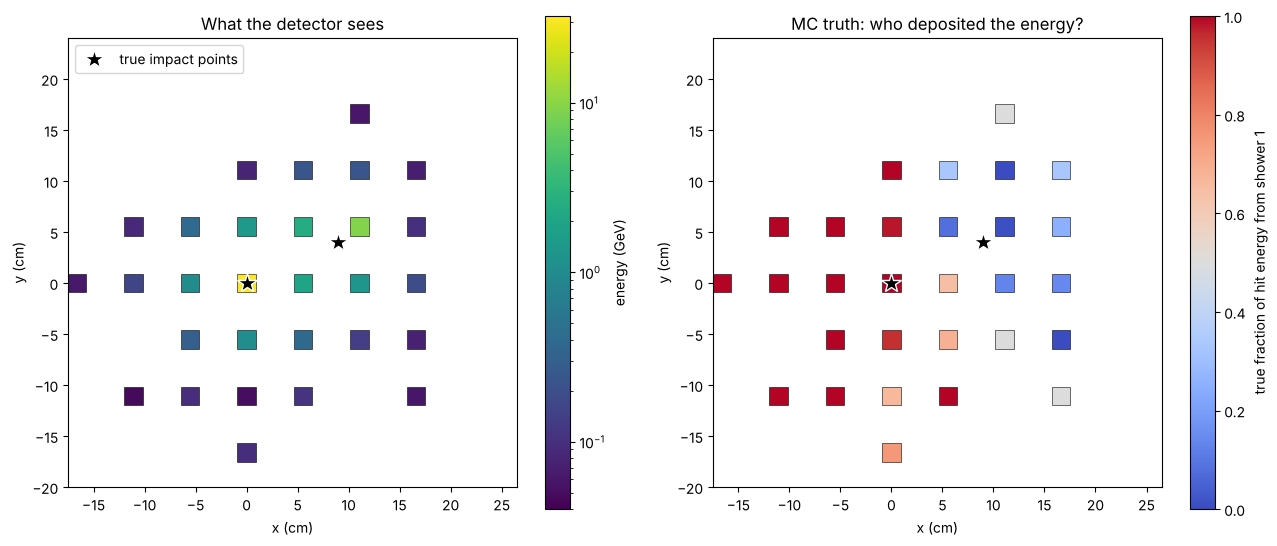
\includegraphics[width=0.92\textwidth]{toy_event_truth.png}
\caption{A toy event with two overlapping showers (40 and 15~GeV). Left: measured tower energies. Right: Monte-Carlo truth --- the fraction of each tower's energy deposited by shower~1.
Towers in between contain energy from both showers, which a hard assignment cannot describe.}
\label{fig:toy}
\end{figure}

\subsection*{A VAE for shower images}

For Problems~4.3 and 4.4 a data point is a whole shower: the $7\times7$ tower energies around the seed, normalised to a sum of one (\cref{fig:windows}).
The VAE has a Gaussian encoder $q_\phi(z|x)=\mathcal{N}(\mu_\phi(x),\mathrm{diag}\,\sigma^2_\phi(x))$, a prior $p(z)=\mathcal{N}(0,\mathbb{I})$ and a decoder that predicts the energy fraction $p_j(z)$ of every tower.
Assuming the energy arrives in $N_q$ independent ``quanta'' gives a multinomial likelihood, and the loss per shower is
\begin{equation}
\mathcal{L}(x)= -N_q\sum_j x_j\log p_j(z) \;+\; \tfrac12\sum_l\big(\mu_l^2+\sigma_l^2-\log\sigma_l^2-1\big),
\qquad z=\mu+\sigma\odot\varepsilon,\;\; \varepsilon\sim\mathcal{N}(0,\mathbb{I}).
\end{equation}
The \emph{reparametrisation} $z=\mu+\sigma\odot\varepsilon$ moves the randomness into an input, so that gradients can flow through the sampling step.
The VAE is written in plain NumPy, so that every term of the loss and of its gradient is visible.

\begin{figure}[h]
\centering
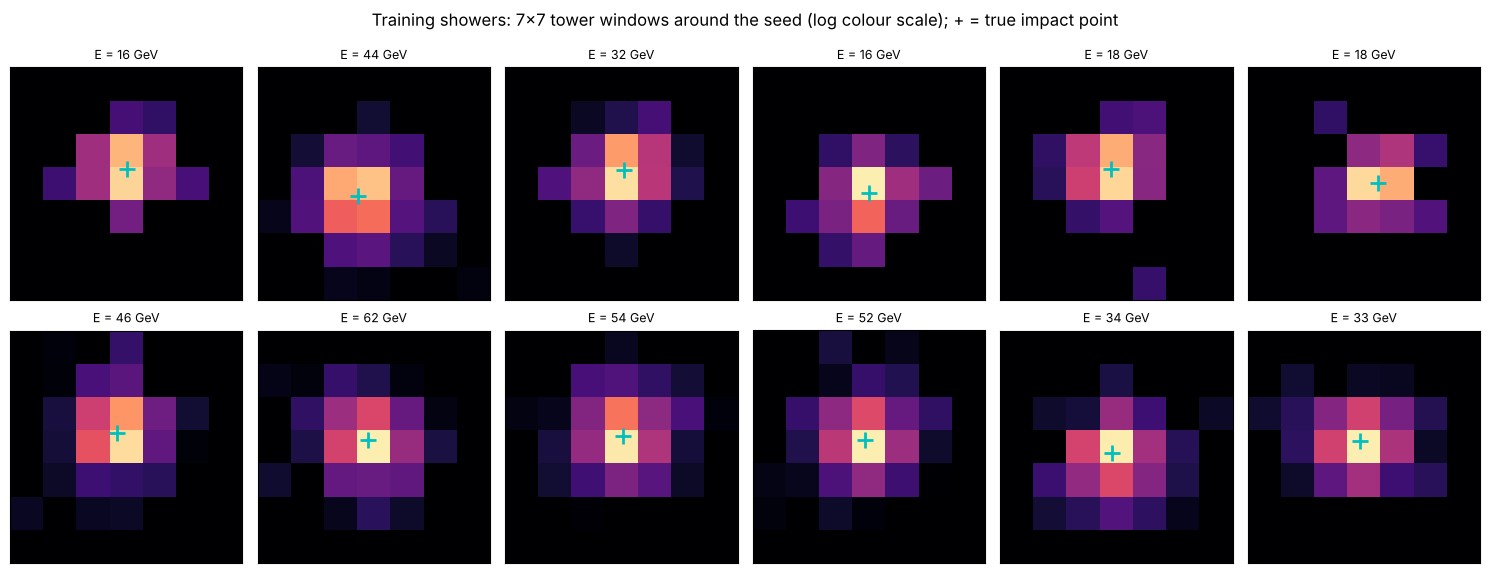
\includegraphics[width=0.95\textwidth]{shower_windows.png}
\caption{Training data for Problems~4.3 and 4.4: $7\times 7$ tower windows around the seed tower of simulated electromagnetic showers (logarithmic colour scale); the cross marks the true impact point.}
\label{fig:windows}
\end{figure}

\subsection*{Your tasks in Section 4}

The PHENIX samples contain no information about which particle produced which hit, and too few events to train a network.
The notebook therefore provides a fast toy simulation with full Monte-Carlo truth, tuned to the shower containment of the PHENIX electrons:
\texttt{ex3.generate\_shower\_event} (events with several showers) and \texttt{ex3.make\_shower\_images} (shower windows).
Only four cells require your code (marked \texttt{\# --> TODO}); the analysis and plotting cells are provided, so concentrate on interpreting the plots.
\begin{description}
\item[Problem 4.1] Energy-weighted $k$-means, seeded with your \texttt{seed\_search}: compare the position resolution with the unweighted version and with the seed-tower centre.
\item[Problem 4.2] Implement the E-step, M-step and ELBO of an energy-weighted Gaussian mixture (unit test provided).
Visualise EM as coordinate ascent on the ELBO, show that $k$-means is its $\sigma\to0$ limit, study the energy sharing as a function of the shower separation, choose $K$ with the BIC, and apply the method to real $A'\to e^+e^-$ events.
\item[Problem 4.3] Use your $k$-means class on 49-dimensional shower vectors: interpret the codebook of shower templates, use it as an autoencoder and study how much information a code of $\log_2 K$ bits carries.
\item[Problem 4.4] Implement the reparametrisation, the KL term and the reconstruction loss (with gradients) of a VAE, train it (about a minute on a CPU) and explore the latent space,
the decoded shower manifold, the generation of new showers and the use of the ELBO to detect merged clusters.
\end{description}

\subsection*{Further reading}
\begin{itemize}\setlength\itemsep{0pt}
\item D.~P.~Kingma, M.~Welling, \emph{Auto-Encoding Variational Bayes}, ICLR 2014, \href{https://arxiv.org/abs/1312.6114}{arXiv:1312.6114}.
\item R.~M.~Neal, G.~E.~Hinton, \emph{A view of the EM algorithm that justifies incremental, sparse, and other variants}, in \emph{Learning in Graphical Models}, Springer, 1998.
\item T.~Hastie, R.~Tibshirani, J.~Friedman, \emph{The Elements of Statistical Learning}, Springer (Sec.~8.5: the EM algorithm).
\item A.~van den Oord, O.~Vinyals, K.~Kavukcuoglu, \emph{Neural Discrete Representation Learning} (VQ-VAE), NeurIPS 2017, \href{https://arxiv.org/abs/1711.00937}{arXiv:1711.00937}.
\item G.~Grindhammer, S.~Peters, \emph{The parameterized simulation of electromagnetic showers in homogeneous and sampling calorimeters}, \href{https://arxiv.org/abs/hep-ex/0001020}{arXiv:hep-ex/0001020}.
\item E.~Nalisnick et al., \emph{Do Deep Generative Models Know What They Don't Know?}, ICLR 2019, \href{https://arxiv.org/abs/1810.09136}{arXiv:1810.09136}.
\end{itemize}

\end{document}
